% !TeX encoding = UTF-8
% !TeX program = pdflatex

%----------------------------------------------------------------------------------------
%    PACKAGES AND OTHER DOCUMENT CONFIGURATIONS
%----------------------------------------------------------------------------------------

\documentclass[paper=a4, fontsize=11pt]{scrartcl} % A4 paper and 11pt font size

\usepackage[utf8]{inputenc}
\usepackage{hyperref}
\usepackage{graphicx}
\usepackage[dvipsnames]{xcolor}   % for \textcolor

\usepackage{pgfplots}
\pgfplotsset{compat=1.13}

\usepackage[T1]{fontenc} % Use 8-bit encoding that has 256 glyphs
%\usepackage{fourier} % Use the Adobe Utopia font for the document - comment this line to return to the LaTeX default
%\usepackage[english]{babel} % English language/hyphenation
\usepackage{amsmath,amsfonts,amsthm} % Math packages

\usepackage{sectsty} % Allows customizing section commands
\allsectionsfont{\centering \normalfont\scshape} % Make all sections centered, the default font and small caps

\usepackage{fancyhdr} % Custom headers and footers
\pagestyle{fancyplain} % Makes all pages in the document conform to the custom headers and footers
\fancyhead{} % No page header - if you want one, create it in the same way as the footers below
\fancyfoot[L]{} % Empty left footer
\fancyfoot[C]{} % Empty center footer
\fancyfoot[R]{\thepage} % Page numbering for right footer
\renewcommand{\headrulewidth}{0pt} % Remove header underlines
\renewcommand{\footrulewidth}{0pt} % Remove footer underlines
\setlength{\headheight}{13.6pt} % Customize the height of the header

\numberwithin{equation}{section} % Number equations within sections (i.e. 1.1, 1.2, 2.1, 2.2 instead of 1, 2, 3, 4)
\numberwithin{figure}{section} % Number figures within sections (i.e. 1.1, 1.2, 2.1, 2.2 instead of 1, 2, 3, 4)
\numberwithin{table}{section} % Number tables within sections (i.e. 1.1, 1.2, 2.1, 2.2 instead of 1, 2, 3, 4)

\setlength\parindent{0pt} % Removes all indentation from paragraphs - comment this line for an assignment with lots of text

\renewcommand{\baselinestretch}{1.10} 

\hypersetup{
    colorlinks,
    citecolor=black,
    filecolor=black,
    linkcolor=black,
    urlcolor=black
}

\makeatletter
\def\BState{\State\hskip-\ALG@thistlm}
\makeatother

\newcommand{\horrule}[1]{\rule{\linewidth}{#1}} % Create horizontal rule command with 1 argument of height

\title{    
\normalfont \normalsize 
\textsc{Machine Learning 2nd Homework - Sapienza University of Rome} \\ [25pt] % Your university, school and/or department name(s)
\horrule{0.5pt} \\[0.4cm] % Thin top horizontal rule
\huge Venice Boat Classification \\ % The assignment title
\horrule{2pt} \\[0.5cm] % Thick bottom horizontal rule
}

\author{Andrea Fioraldi 1692419} % Your name

\date{\normalsize\today} % Today's date or a custom date

\begin{document}

\maketitle % Print the title

\section*{The Problem}

We want to construct a model to classify images that contain boats of Venice or does not contain boats.

We used the {\em ARGOS} training set to train several neural networks and then a preprocessed version of the test set for the validation.

The classes are 24:

\begin{verbatim}
Alilaguna, Ambulanza, Barchino, Cacciapesca, Caorlina, Gondola, Lanciafino10m,
Lanciafino10mBianca, Lanciafino10mMarrone, Lanciamaggioredi10mBianca,
Lanciamaggioredi10mMarrone, Motobarca, Motopontonerettangolare, MotoscafoACTV,
Mototopo, Patanella, Polizia, Raccoltarifiuti, Sandoloaremi, Sanpierota, Topa,
VaporettoACTV, VigilidelFuoco, Water
\end{verbatim}

The size of each image is 800x240.

We chose {\em keras} as the library for such networks.

\section*{Preprocessing}

From the training set we removed all the images with a class that is not present in the training set:
\begin{itemize}
    \item \verb|Mototopo corto|;
    \item \verb|Snapshot Barca Multipla|;
    \item \verb|Snapshot Barca Parziale|;
\end{itemize}
We renamed the \verb|Snapshot Acqua| class of the test set to \verb|Water| to match the train set.

The training dataset directory structure is compatible with keras but this is not true for the test set, so we created a directory compatible with the automated images preprocessing functions of keras.
We added also empty folders in order to indicate that a class has no images in the test set.

The directory structure is the following:

\begin{itemize}
    \item \verb|sc5_test|
    \begin{itemize}
        \item \verb|class0|
        \begin{itemize}
            \item \verb|image0_class0.jpeg|
            \item ...
            \item \verb|imageN_class0.jpeg|
        \end{itemize}
        \item ...
        \item \verb|class24|
        \begin{itemize}
            \item \verb|image0_class24.jpeg|
            \item ...
            \item \verb|imageN_class24.jpeg|
        \end{itemize}
    \end{itemize}
\end{itemize}

We exploited this directory structure in order to use the {\em ImageDataGenerator} class of keras for automated image loading and preprocessing.
All the images are loaded in color mode RGB with batch size 32.
The target size of ImageDataGenerator is one of the parameters that we changed in the experiments. When this parameter is present, the images are stretched to the target size.

After all, in the training set we have 4774 images and in the test set 1672 images.

\section*{Classification}

The metrics that we used for the classifications are the accuracy and the loss function.
The chosen loss function is the Categorical Crossentropy, a logarithmic function that increases when the prediction is far from the label, so it must be kept as lower as possible.

We trained the networks using a GeForce GTX 1050 with 1.5 GHz clock and 4 Gb of memory.

\section*{Well-Known Networks}

We used different neural networks for this classification problem.

In the beginning, we chose two well-known networks, LeNet and AlexNet.

\subsection*{LeNet}

Input shape: 320x320.

Parameters:
\begin{itemize}
    \item Total params: 55,251,196;
    \item Trainable params: 55,251,196;
    \item Non-trainable params: 0;
\end{itemize}

\bigskip
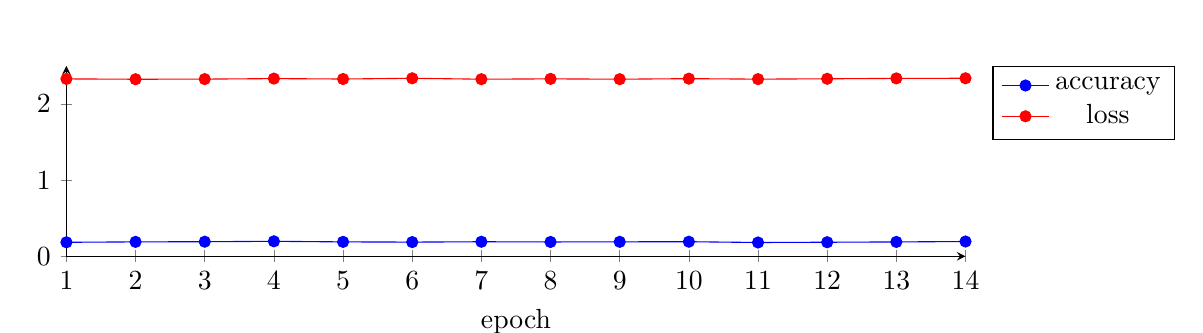
\begin{tikzpicture}
    \begin{axis}[
        width=13cm, height=4cm,
        ymin=0, ymax=2.5,
        xmin=1, xmax=14,
        axis x line=bottom,
        axis y line=left,
        xlabel=epoch,
        title={},
        axis on top=true, clip=false,
        legend pos=outer north east
    ]
    \addplot[mark=*, blue] coordinates {
        (1, 0.1838) (2, 0.1891) (3, 0.1913) (4, 0.1965) (5, 0.1890) (6, 0.1862) (7, 0.1907) (8, 0.1880) (9, 0.1897) (10, 0.1913) (11, 0.1810) (12, 0.1844) (13, 0.1884) (14, 0.1940)
    };
    \addplot[mark=*, red] coordinates {
        (1, 2.3287) (2, 2.3244) (3, 2.3260) (4, 2.3326) (5, 2.3273) (6, 2.3369) (7, 2.3249) (8, 2.3292) (9, 2.3249) (10, 2.3319) (11, 2.3256) (12, 2.3302) (13, 2.3355) (14, 2.3370)
    };
    \addlegendentry{accuracy}
    \addlegendentry{loss}
    \end{axis}
\end{tikzpicture}
\bigskip

Training time: 17.750000 minutes.

Final epoch performance:
\begin{itemize}
    \item Loss: 2.3370;
    \item Accuracy: 0.1940;
\end{itemize}

Test set performance:
\begin{itemize}
    \item Loss: 2.202084;
    \item Accuracy: 0.192909;
\end{itemize}

In each epoch the gain of this net is very poor we stopped the training after 14 epochs.

The performance is very bad so we do not test other configurations with LeNet and switched to AlexNet.

\subsection*{AlexNet}

Input shape: 320x320.

Parameters:
\begin{itemize}
    \item Total params: 43,832,416;
    \item Trainable params: 43,811,280;
    \item Non-trainable params: 21,136;
\end{itemize}

\bigskip
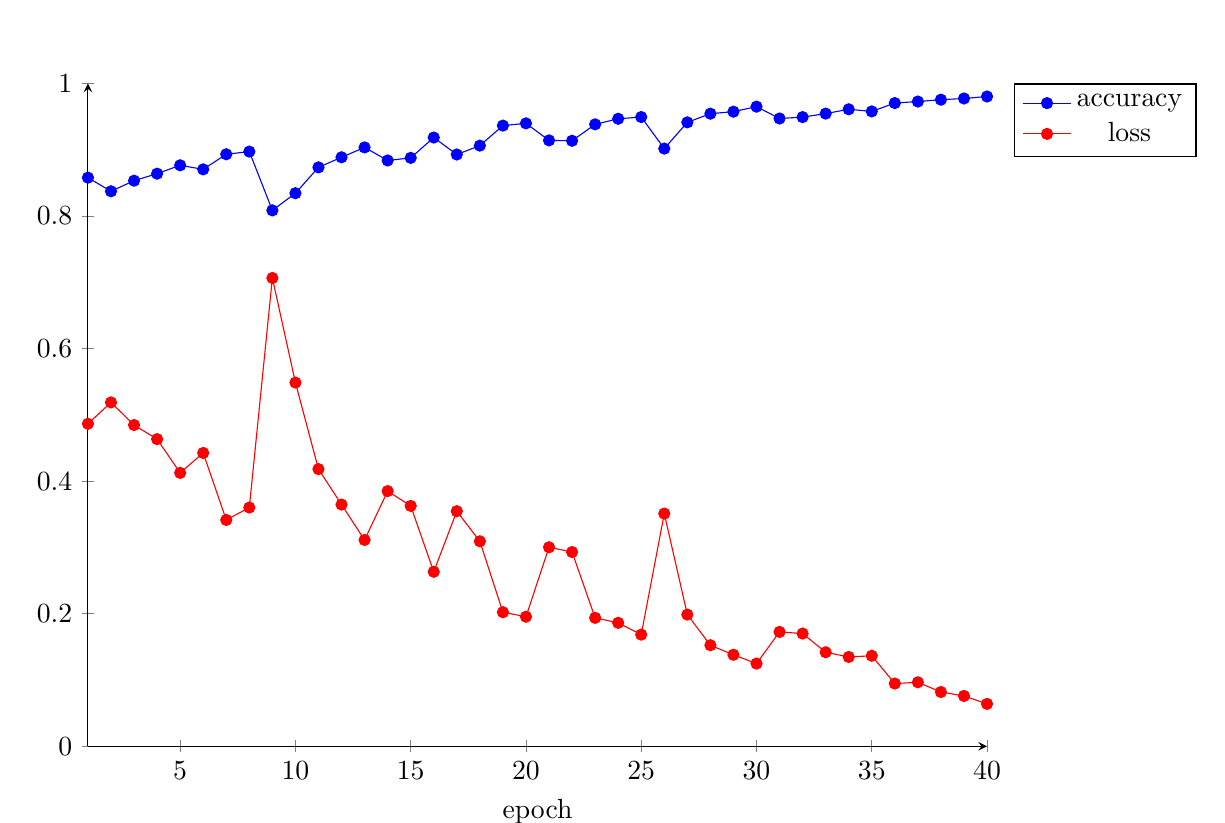
\begin{tikzpicture}
    \begin{axis}[
        width=13cm, height=10cm,
        ymin=0, ymax=1,
        xmin=1, xmax=40,
        axis x line=bottom,
        axis y line=left,
        xlabel=epoch,
        title={},
        axis on top=true, clip=false,
        legend pos=outer north east
    ]
    \addplot[mark=*, blue] coordinates {
        (1, 0.8579) (2, 0.8373) (3, 0.8533) (4, 0.8639) (5, 0.8765) (6, 0.8704) (7, 0.8932) (8, 0.8972) (9, 0.8085) (10, 0.8344) (11, 0.8734) (12, 0.8886) (13, 0.9035) (14, 0.8838) (15, 0.8877) (16, 0.9184) (17, 0.8928) (18, 0.9062) (19, 0.9364) (20, 0.9398) (21, 0.9141) (22, 0.9135) (23, 0.9383) (24, 0.9467) (25, 0.9493) (26, 0.9017) (27, 0.9413) (28, 0.9544) (29, 0.9574) (30, 0.9650) (31, 0.9471) (32, 0.9492) (33, 0.9545) (34, 0.9610) (35, 0.9578) (36, 0.9704) (37, 0.9727) (38, 0.9755) (39, 0.9773) (40, 0.9803)
    };
    \addplot[mark=*, red] coordinates {
        (1, 0.4866) (2, 0.5188) (3, 0.4847) (4, 0.4634) (5, 0.4125) (6, 0.4426) (7, 0.3415) (8, 0.3602) (9, 0.7065) (10, 0.5487) (11, 0.4182) (12, 0.3647) (13, 0.3113) (14, 0.3850) (15, 0.3627) (16, 0.2633) (17, 0.3547) (18, 0.3093) (19, 0.2023) (20, 0.1955) (21, 0.3003) (22, 0.2931) (23, 0.1938) (24, 0.1863) (25, 0.1685) (26, 0.3511) (27, 0.1987) (28, 0.1525) (29, 0.1381) (30, 0.1248) (31, 0.1726) (32, 0.1701) (33, 0.1419) (34, 0.1348) (35, 0.1366) (36, 0.0947) (37, 0.0966) (38, 0.0819) (39, 0.0760) (40, 0.0640)
    };
    \addlegendentry{accuracy}
    \addlegendentry{loss}
    \end{axis}
\end{tikzpicture}
\bigskip

Training time: 31.416667 minutes.

Final epoch performance:
\begin{itemize}
    \item Loss: 0.0640;
    \item Accuracy: 0.9803;
\end{itemize}

Test set performance:
\begin{itemize}
    \item Loss: 1.190347;
    \item Accuracy: 0.810096;
\end{itemize}

AlexNet seems a good model.
The performance on the test set are not as good as the performance on the train set but this is quite obvious.

81% of accuracy is great for a network trained on such small dataset.
Loss is quite high but tolerable.

We also tried to enlarge the input shape.

\bigskip
Input shape: 420x420.
Parameters:
\begin{itemize}
    \item Total params: 78,435,424;
    \item Trainable params: 78,414,288;
    \item Non-trainable params: 21,136;
\end{itemize}

\bigskip
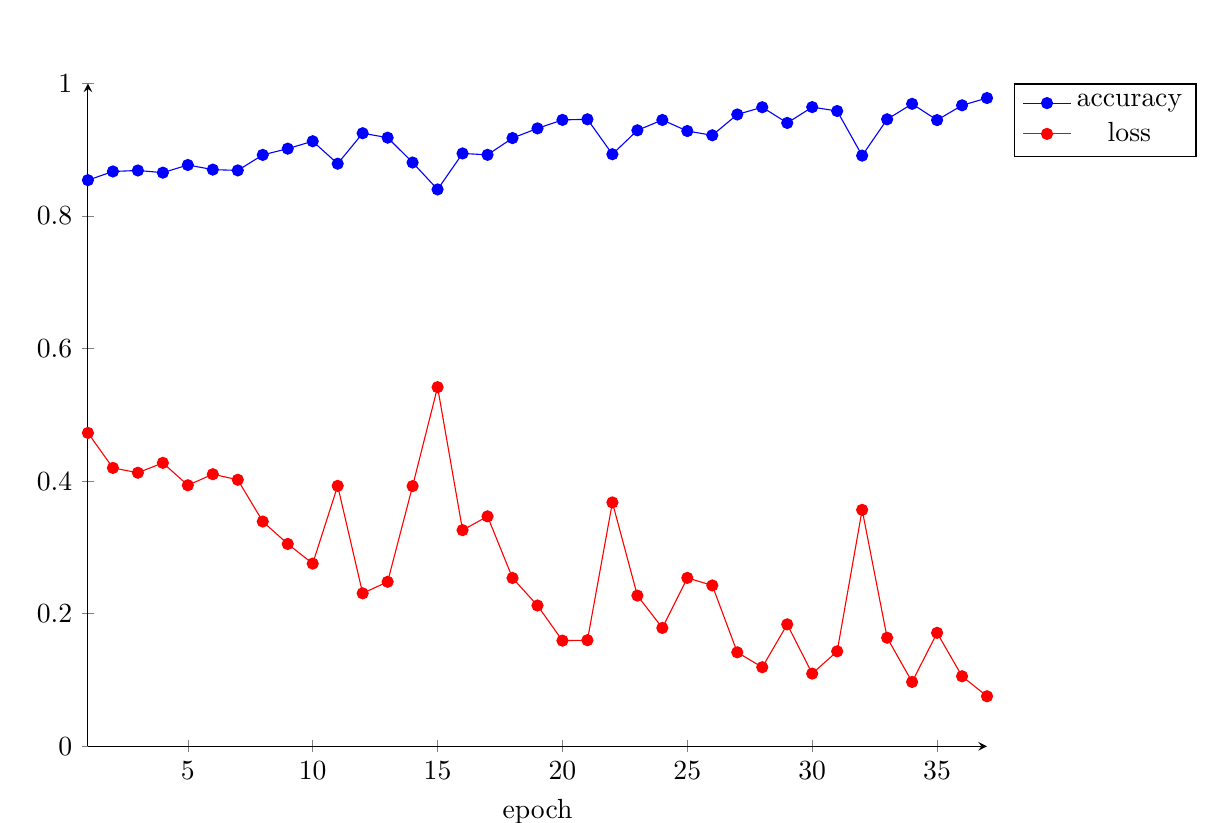
\begin{tikzpicture}
    \begin{axis}[
        width=13cm, height=10cm,
        ymin=0, ymax=1,
        xmin=1, xmax=37,
        axis x line=bottom,
        axis y line=left,
        xlabel=epoch,
        title={},
        axis on top=true, clip=false,
        legend pos=outer north east
    ]
    \addplot[mark=*, blue] coordinates {
        (1, 0.8541) (2, 0.8672) (3, 0.8687) (4, 0.8654) (5, 0.8770) (6, 0.8700) (7, 0.8688) (8, 0.8922) (9, 0.9016) (10, 0.9128) (11, 0.8789) (12, 0.9249) (13, 0.9182) (14, 0.8807) (15, 0.8401) (16, 0.8944) (17, 0.8923) (18, 0.9176) (19, 0.9322) (20, 0.9450) (21, 0.9459) (22, 0.8932) (23, 0.9293) (24, 0.9449) (25, 0.9282) (26, 0.9218) (27, 0.9532) (28, 0.9641) (29, 0.9404) (30, 0.9643) (31, 0.9584) (32, 0.8911) (33, 0.9459) (34, 0.9692) (35, 0.9447) (36, 0.9670) (37, 0.9780)
    };
    \addplot[mark=*, red] coordinates {
        (1, 0.4728) (2, 0.4200) (3, 0.4127) (4, 0.4276) (5, 0.3938) (6, 0.4105) (7, 0.4021) (8, 0.3391) (9, 0.3053) (10, 0.2756) (11, 0.3929) (12, 0.2308) (13, 0.2482) (14, 0.3926) (15, 0.5418) (16, 0.3261) (17, 0.3469) (18, 0.2539) (19, 0.2124) (20, 0.1594) (21, 0.1601) (22, 0.3679) (23, 0.2274) (24, 0.1786) (25, 0.2541) (26, 0.2427) (27, 0.1418) (28, 0.1193) (29, 0.1840) (30, 0.1097) (31, 0.1433) (32, 0.3567) (33, 0.1638) (34, 0.0971) (35, 0.1712) (36, 0.1057) (37, 0.0755)
    };
    \addlegendentry{accuracy}
    \addlegendentry{loss}
    \end{axis}
\end{tikzpicture}
\bigskip

Training time: 72.516667 minutes.

Final epoch performance:
\begin{itemize}
    \item Loss: 0.0755;
    \item Accuracy: 0.9780;
\end{itemize}

Test set performance:
\begin{itemize}
    \item Loss: 0.866917;
    \item Accuracy: 0.839543;
\end{itemize}

As you can see in the graph, using such input size the accuracy and the loss is more unstable in time.
Probably we stopped too early the training and the network needs a greater number of epoch to converge.
Despite this, the result is better than the first run.

\subsection*{Why not other known networks?}

We tried also the Inception networks from Google but they are too complex for our hardware.
The GPU memory goes full almost immediately.

\section*{AndreaNet}

After using the known networks we decided to create a custom network called AndreaNet.

As seen before, LeNet is a bad model on this dataset so we started from it with the aim to create a net with performance comparable with AlexNet.

We created 3 versions of AndreaNet with different parameters tuning and in the end, it is a completely new neural network.

\subsection**{Version 1}

This is the diff of the LeNet layers and AndreaNet v1 layers:

\bigskip
\begin{tabular}{ | l | l | }
    \hline
    \textbf{LeNet} & \textbf{AndreaNet v1} \\ \hline
    Convolutional 6 kernels 5x5 & Convolutional 6 kernels 11x11 \\ \hline 
    Average Pooling 2x2 stride 2x2 & Average Pooling 2x2 stride 2x2 \\ \hline 
    Convolutional 16 kernels 5x5 & Convolutional 16 kernels 8x8 \\ \hline 
    Average Pooling 2x2 stride 2x2 & Average Pooling 2x2 stride 2x2 \\ \hline
    Convolutional 120 kernels 5x5 & Convolutional 120 kernels 8x8 \\ \hline
    & Average Pooling 2x2 stride 2x2 \\ \hline     
    & Convolutional 240 kernels 2x2 \\ \hline 
    Fully connected, 84 units & Fully connected, 2048 units (dropout 0.5) \\ \hline 
    & Fully connected, 512 units \\ \hline 
    Fully connected, 24 units & Fully connected, 24 units \\ \hline 
\end{tabular}
\bigskip

All of them uses the tanh activation function except for the last that uses softmax, as in LeNet.

As you can see in the diff we enlarged the size of kernels to test if this can be a tuning that allows the net to perform better.
After all layers, we also added BatchNormalization, one of the advantages of AlexNet, and this helped us to create a deeper network that is, generally, better.
We also added a convolutional layer and a larger dense layer for the creation of a deeper network.
\bigskip
Input shape: 320x320.

Parameters:
\begin{itemize}
    \item Total params: 3,288,080;
    \item Trainable params: 3,282,196;
    \item Non-trainable params: 5,884;
\end{itemize}

\bigskip
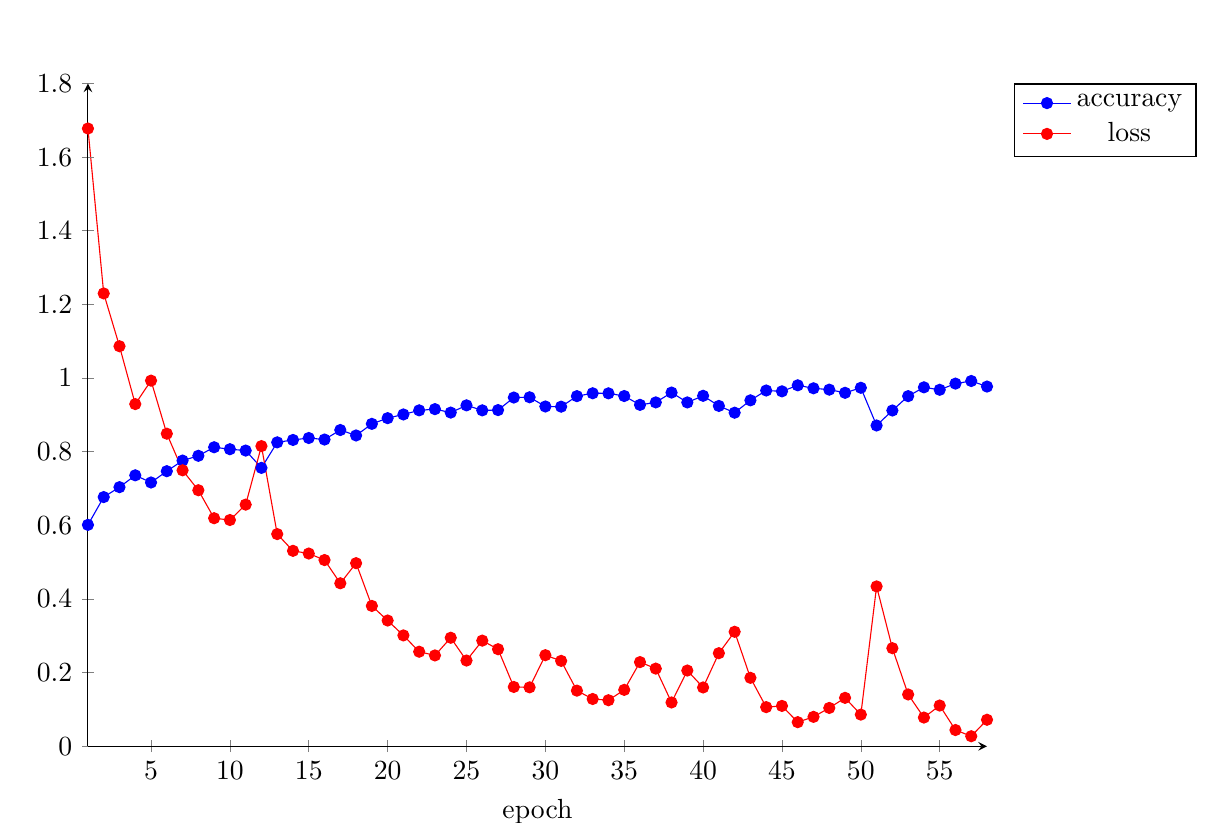
\begin{tikzpicture}
    \begin{axis}[
        width=13cm, height=10cm,
        ymin=0, ymax=1.8,
        xmin=1, xmax=58,
        axis x line=bottom,
        axis y line=left,
        xlabel=epoch,
        title={},
        axis on top=true, clip=false,
        legend pos=outer north east
    ]
    \addplot[mark=*, blue] coordinates {
        (1, 0.6013) (2, 0.6768) (3, 0.7037) (4, 0.7359) (5, 0.7164) (6, 0.7471) (7, 0.7759) (8, 0.7889) (9, 0.8121) (10, 0.8068) (11, 0.8031) (12, 0.7561) (13, 0.8254) (14, 0.8319) (15, 0.8372) (16, 0.8330) (17, 0.8589) (18, 0.8441) (19, 0.8756) (20, 0.8911) (21, 0.9012) (22, 0.9123) (23, 0.9156) (24, 0.9062) (25, 0.9259) (26, 0.9123) (27, 0.9130) (28, 0.9471) (29, 0.9478) (30, 0.9228) (31, 0.9223) (32, 0.9509) (33, 0.9587) (34, 0.9585) (35, 0.9512) (36, 0.9272) (37, 0.9339) (38, 0.9606) (39, 0.9338) (40, 0.9518) (41, 0.9243) (42, 0.9059) (43, 0.9395) (44, 0.9662) (45, 0.9639) (46, 0.9803) (47, 0.9722) (48, 0.9685) (49, 0.9599) (50, 0.9736) (51, 0.8712) (52, 0.9119) (53, 0.9509) (54, 0.9748) (55, 0.9681) (56, 0.9849) (57, 0.9920) (58, 0.9769)
    };
    \addplot[mark=*, red] coordinates {
        (1, 1.6776) (2, 1.2298) (3, 1.0864) (4, 0.9293) (5, 0.9930) (6, 0.8489) (7, 0.7495) (8, 0.6954) (9, 0.6194) (10, 0.6145) (11, 0.6563) (12, 0.8152) (13, 0.5763) (14, 0.5308) (15, 0.5235) (16, 0.5058) (17, 0.4427) (18, 0.4973) (19, 0.3812) (20, 0.3416) (21, 0.3012) (22, 0.2569) (23, 0.2468) (24, 0.2948) (25, 0.2329) (26, 0.2870) (27, 0.2637) (28, 0.1612) (29, 0.1601) (30, 0.2475) (31, 0.2320) (32, 0.1512) (33, 0.1285) (34, 0.1252) (35, 0.1533) (36, 0.2287) (37, 0.2110) (38, 0.1191) (39, 0.2058) (40, 0.1598) (41, 0.2529) (42, 0.3110) (43, 0.1860) (44, 0.1064) (45, 0.1097) (46, 0.0656) (47, 0.0800) (48, 0.1042) (49, 0.1316) (50, 0.0861) (51, 0.4342) (52, 0.2665) (53, 0.1408) (54, 0.0781) (55, 0.1108) (56, 0.0442) (57, 0.0274) (58, 0.0721)
    };
    \addlegendentry{accuracy}
    \addlegendentry{loss}
    \end{axis}
\end{tikzpicture}
\bigskip

Training time: 15.716667 minutes.

Final epoch performance:
\begin{itemize}
    \item Loss: 0.0721;
    \item Accuracy: 0.9769;
\end{itemize}

Test set performance:
\begin{itemize}
    \item Loss: 1.466683;
    \item Accuracy: 0.767428;
\end{itemize}

The results are very good respect LeNet. We also tried to get better results enlarging the input shape.
\bigskip
Input shape: 420x420.

Parameters:
\begin{itemize}
    \item Total params: 5,745,680;
    \item Trainable params: 5,739,796;
    \item Non-trainable params: 5,884;
\end{itemize}

\bigskip
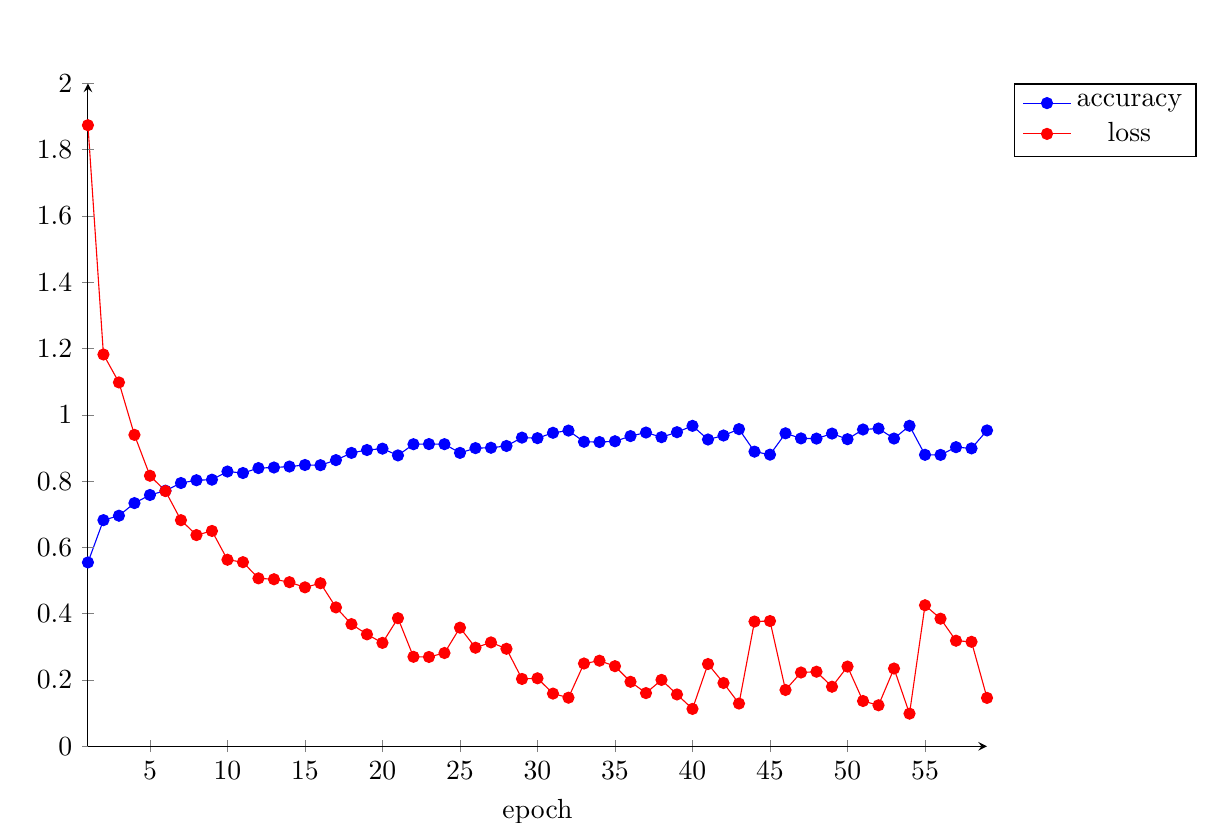
\begin{tikzpicture}
    \begin{axis}[
        width=13cm, height=10cm,
        ymin=0, ymax=2,
        xmin=1, xmax=59,
        axis x line=bottom,
        axis y line=left,
        xlabel=epoch,
        title={},
        axis on top=true, clip=false,
        legend pos=outer north east
    ]
    \addplot[mark=*, blue] coordinates {
        (1, 0.5548) (2, 0.6824) (3, 0.6958) (4, 0.7338) (5, 0.7583) (6, 0.7713) (7, 0.7944) (8, 0.8028) (9, 0.8045) (10, 0.8291) (11, 0.8246) (12, 0.8395) (13, 0.8412) (14, 0.8441) (15, 0.8488) (16, 0.8482) (17, 0.8635) (18, 0.8853) (19, 0.8940) (20, 0.8981) (21, 0.8777) (22, 0.9115) (23, 0.9119) (24, 0.9116) (25, 0.8853) (26, 0.8997) (27, 0.9008) (28, 0.9062) (29, 0.9314) (30, 0.9297) (31, 0.9459) (32, 0.9526) (33, 0.9188) (34, 0.9180) (35, 0.9204) (36, 0.9360) (37, 0.9467) (38, 0.9327) (39, 0.9478) (40, 0.9669) (41, 0.9257) (42, 0.9377) (43, 0.9570) (44, 0.8891) (45, 0.8800) (46, 0.9444) (47, 0.9290) (48, 0.9284) (49, 0.9436) (50, 0.9266) (51, 0.9559) (52, 0.9588) (53, 0.9286) (54, 0.9671) (55, 0.8795) (56, 0.8793) (57, 0.9026) (58, 0.8989) (59, 0.9531)
    };
    \addplot[mark=*, red] coordinates {
        (1, 1.8740) (2, 1.1822) (3, 1.0979) (4, 0.9397) (5, 0.8164) (6, 0.7701) (7, 0.6823) (8, 0.6373) (9, 0.6498) (10, 0.5629) (11, 0.5556) (12, 0.5068) (13, 0.5041) (14, 0.4952) (15, 0.4796) (16, 0.4921) (17, 0.4191) (18, 0.3687) (19, 0.3378) (20, 0.3121) (21, 0.3866) (22, 0.2701) (23, 0.2696) (24, 0.2815) (25, 0.3580) (26, 0.2975) (27, 0.3135) (28, 0.2943) (29, 0.2033) (30, 0.2052) (31, 0.1591) (32, 0.1467) (33, 0.2498) (34, 0.2583) (35, 0.2418) (36, 0.1947) (37, 0.1606) (38, 0.2004) (39, 0.1565) (40, 0.1129) (41, 0.2483) (42, 0.1911) (43, 0.1290) (44, 0.3765) (45, 0.3780) (46, 0.1700) (47, 0.2227) (48, 0.2251) (49, 0.1798) (50, 0.2406) (51, 0.1367) (52, 0.1238) (53, 0.2347) (54, 0.0986) (55, 0.4256) (56, 0.3851) (57, 0.3186) (58, 0.3153) (59, 0.1461)
    };
    \addlegendentry{accuracy}
    \addlegendentry{loss}
    \end{axis}
\end{tikzpicture}
\bigskip

Training time: 66.366667 minutes.

Final epoch performance:
\begin{itemize}
    \item Loss: 0.1461;
    \item Accuracy: 0.9531;
\end{itemize}

Test set performance:
\begin{itemize}
    \item Loss: 0.999524;
    \item Accuracy: 0.802284;
\end{itemize}

These results are very near to the results of AlexNet.

\subsection*{Version 2}

In order to perform even better than AndreaNet v1 we created a second version.
We maintained the layer structure of the v1 but we changed all the activation functions of the convolutional layers to ReLU.
We also have chosen to try the SGD optimizer so we replaced adam with it.

Parameters:
\begin{itemize}
    \item Total params: 3,288,080;
    \item Trainable params: 3,282,196;
    \item Non-trainable params: 5,884;
\end{itemize}

\bigskip
\begin{tikzpicture}
    \begin{axis}[
        width=13cm, height=10cm,
        ymin=0, ymax=1.8,
        xmin=1, xmax=28,
        axis x line=bottom,
        axis y line=left,
        xlabel=epoch,
        title={},
        axis on top=true, clip=false,
        legend pos=outer north east
    ]
    \addplot[mark=*, blue] coordinates {
        (1, 0.6026) (2, 0.6947) (3, 0.7362) (4, 0.7634) (5, 0.7924) (6, 0.8097) (7, 0.8375) (8, 0.8586) (9, 0.8674) (10, 0.8953) (11, 0.9010) (12, 0.9167) (13, 0.9297) (14, 0.9268) (15, 0.9502) (16, 0.9526) (17, 0.9579) (18, 0.9740) (19, 0.9779) (20, 0.9786) (21, 0.9880) (22, 0.9815) (23, 0.9806) (24, 0.9910) (25, 0.9768) (26, 0.9868) (27, 0.9952) (28, 0.9897)
    };
    \addplot[mark=*, red] coordinates {
        (1, 1.5932) (2, 1.1176) (3, 0.9379) (4, 0.8369) (5, 0.6950) (6, 0.6284) (7, 0.5265) (8, 0.4672) (9, 0.4269) (10, 0.3536) (11, 0.3081) (12, 0.2696) (13, 0.2227) (14, 0.2387) (15, 0.1737) (16, 0.1476) (17, 0.1381) (18, 0.0988) (19, 0.0805) (20, 0.0805) (21, 0.0560) (22, 0.0650) (23, 0.0669) (24, 0.0412) (25, 0.0823) (26, 0.0550) (27, 0.0301) (28, 0.0441)
    };
    \addlegendentry{accuracy}
    \addlegendentry{loss}
    \end{axis}
\end{tikzpicture}
\bigskip

Training time: 7.983333 minutes.

Final epoch performance:
\begin{itemize}
    \item Loss: 0.0441;
    \item Accuracy: 0.9897;
\end{itemize}

Test set performance:
\begin{itemize}
    \item Loss: 0.988192;
    \item Accuracy: 0.822716;
\end{itemize}

Bingo! The results with input shape 320x320 are even better than the results of AlexNet!
\bigskip
Input shape: 420x420.

Parameters:
\begin{itemize}
    \item Total params: 5,745,680;
    \item Trainable params: 5,739,796;
    \item Non-trainable params: 5,884;
\end{itemize}

\bigskip
\begin{tikzpicture}
    \begin{axis}[
        width=13cm, height=10cm,
        ymin=0, ymax=2,
        xmin=1, xmax=26,
        axis x line=bottom,
        axis y line=left,
        xlabel=epoch,
        title={},
        axis on top=true, clip=false,
        legend pos=outer north east
    ]
    \addplot[mark=*, blue] coordinates {
        (1, 0.6095) (2, 0.7294) (3, 0.7654) (4, 0.7900) (5, 0.8143) (6, 0.8326) (7, 0.8511) (8, 0.8735) (9, 0.8827) (10, 0.9029) (11, 0.9095) (12, 0.9266) (13, 0.9389) (14, 0.9338) (15, 0.9373) (16, 0.9553) (17, 0.9603) (18, 0.9727) (19, 0.9762) (20, 0.9834) (21, 0.9838) (22, 0.9897) (23, 0.9838) (24, 0.9878) (25, 0.9865) (26, 0.9929)
    };
    \addplot[mark=*, red] coordinates {
        (1, 1.5532) (2, 1.0250) (3, 0.8352) (4, 0.7218) (5, 0.6323) (6, 0.5497) (7, 0.4746) (8, 0.4154) (9, 0.3815) (10, 0.3191) (11, 0.2975) (12, 0.2448) (13, 0.1983) (14, 0.2295) (15, 0.2114) (16, 0.1548) (17, 0.1298) (18, 0.1049) (19, 0.0898) (20, 0.0657) (21, 0.0687) (22, 0.0541) (23, 0.0624) (24, 0.0569) (25, 0.0584) (26, 0.0399)
    };
    \addlegendentry{accuracy}
    \addlegendentry{loss}
    \end{axis}
\end{tikzpicture}
\bigskip

Training time: 33.600000 minutes.

Final epoch performance:
\begin{itemize}
    \item Loss: 0.0399;
    \item Accuracy: 0.9929;
\end{itemize}

Test set performance:
\begin{itemize}
    \item Loss: 0.868631;
    \item Accuracy: 0.829327;
\end{itemize}

Enlarging the input shape for version 2 to 420x420 seems to not give a big gain. AlexNet won this round.

\subsection*{Version 3}

In this version, we tried to enlarge the size of the convolutional layers.
We also replaced the activation function of the dense layer to ReLU and changed back the optimizer to adam.

Now the differences between the layers structure from LeNet are very marked:

\bigskip
\begin{tabular}{ | l | l | }
    \hline
    \textbf{LeNet} & \textbf{AndreaNet v3} \\ \hline
    Convolutional 6 kernels 5x5 & Convolutional 12 kernels 11x11 \\ \hline 
    Average Pooling 2x2 stride 2x2 & Average Pooling 2x2 stride 2x2 \\ \hline 
    Convolutional 16 kernels 5x5 & Convolutional 32 kernels 8x8 \\ \hline 
    Average Pooling 2x2 stride 2x2 & Average Pooling 2x2 stride 2x2 \\ \hline
    Convolutional 120 kernels 5x5 & Convolutional 240 kernels 8x8 \\ \hline
    & Average Pooling 2x2 stride 2x2 \\ \hline     
    & Convolutional 360 kernels 2x2 \\ \hline 
    Fully connected, 84 units & Fully connected, 2048 units (dropout 0.5) \\ \hline 
    & Fully connected, 512 units \\ \hline 
    Fully connected, 24 units & Fully connected, 24 units \\ \hline 
\end{tabular}
\bigskip

Input shape: 320x320.

Parameters:
\begin{itemize}
    \item Total params: 4,892,080;
    \item Trainable params: 4,885,672;
    \item Non-trainable params: 6,408;
\end{itemize}

\bigskip
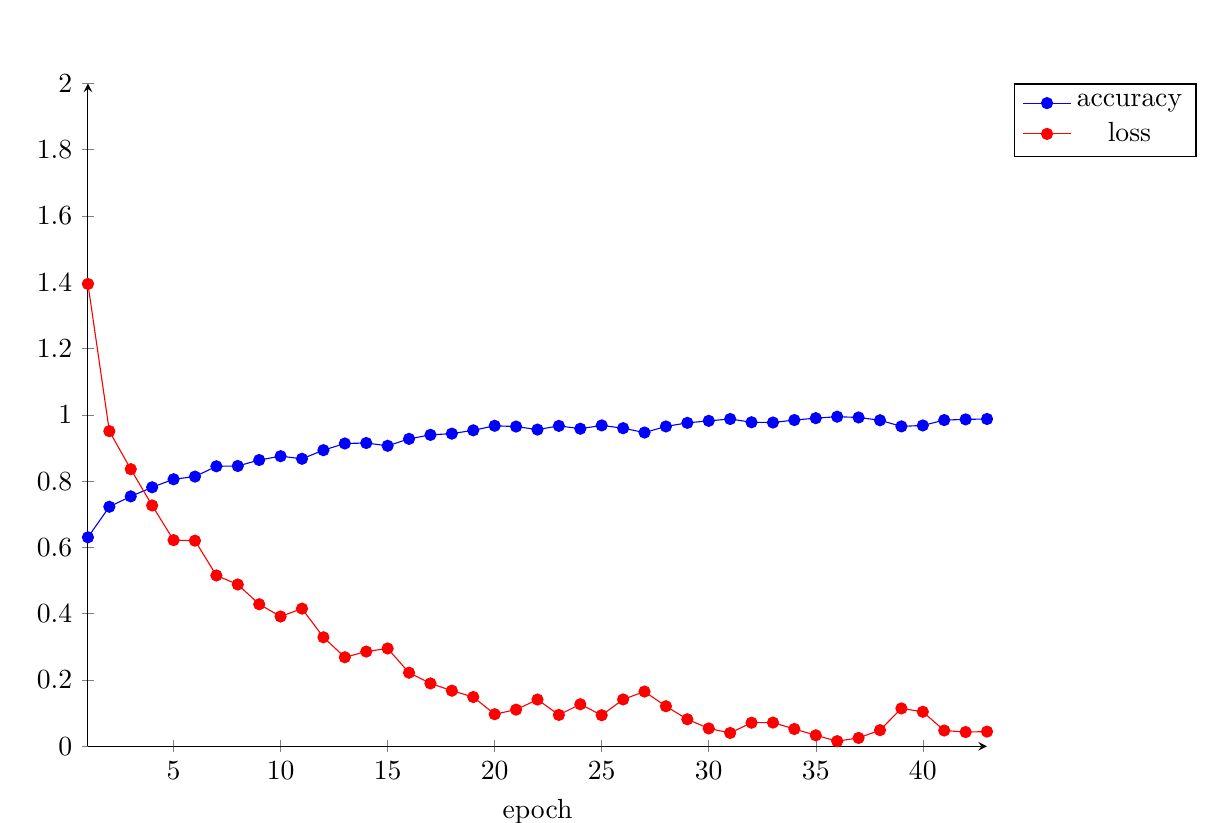
\begin{tikzpicture}
    \begin{axis}[
        width=13cm, height=10cm,
        ymin=0, ymax=2,
        xmin=1, xmax=43,
        axis x line=bottom,
        axis y line=left,
        xlabel=epoch,
        title={},
        axis on top=true, clip=false,
        legend pos=outer north east
    ]
    \addplot[mark=*, blue] coordinates {
        (1, 0.6306) (2, 0.7228) (3, 0.7541) (4, 0.7816) (5, 0.8058) (6, 0.8138) (7, 0.8449) (8, 0.8458) (9, 0.8638) (10, 0.8754) (11, 0.8675) (12, 0.8935) (13, 0.9137) (14, 0.9151) (15, 0.9067) (16, 0.9276) (17, 0.9397) (18, 0.9434) (19, 0.9534) (20, 0.9671) (21, 0.9648) (22, 0.9556) (23, 0.9668) (24, 0.9582) (25, 0.9683) (26, 0.9598) (27, 0.9467) (28, 0.9651) (29, 0.9759) (30, 0.9820) (31, 0.9876) (32, 0.9777) (33, 0.9769) (34, 0.9844) (35, 0.9901) (36, 0.9945) (37, 0.9922) (38, 0.9838) (39, 0.9653) (40, 0.9681) (41, 0.9843) (42, 0.9864) (43, 0.9876)
    };
    \addplot[mark=*, red] coordinates {
        (1, 1.3950) (2, 0.9509) (3, 0.8362) (4, 0.7267) (5, 0.6221) (6, 0.6205) (7, 0.5155) (8, 0.4882) (9, 0.4287) (10, 0.3916) (11, 0.4155) (12, 0.3290) (13, 0.2687) (14, 0.2859) (15, 0.2952) (16, 0.2221) (17, 0.1898) (18, 0.1678) (19, 0.1487) (20, 0.0969) (21, 0.1107) (22, 0.1411) (23, 0.0947) (24, 0.1270) (25, 0.0938) (26, 0.1415) (27, 0.1652) (28, 0.1209) (29, 0.0816) (30, 0.0539) (31, 0.0403) (32, 0.0712) (33, 0.0716) (34, 0.0522) (35, 0.0332) (36, 0.0156) (37, 0.0253) (38, 0.0488) (39, 0.1144) (40, 0.1042) (41, 0.0476) (42, 0.0430) (43, 0.0444)
    };
    \addlegendentry{accuracy}
    \addlegendentry{loss}
    \end{axis}
\end{tikzpicture}
\bigskip

Training time: 14.550000 minutes.

Final epoch performance:
\begin{itemize}
    \item Loss: 0.0444;
    \item Accuracy: 0.9876;
\end{itemize}

Test set performance:
\begin{itemize}
    \item Loss: 1.029947;
    \item Accuracy: 0.844351;
\end{itemize}

We performed even better than AlexNet with input shape 420x420.
Adding a layer instead of enlarging the existing layers is generally preferable, but in this case was a good choice.
The ReLU function is also very good and the gain respect tanh (or sigmoid) is tangible.

For curiosity, we also tried the other input shape.

\bigskip
Input shape: 420x420.

Parameters:
\begin{itemize}
    \item Total params: 8,578,480;
    \item Trainable params: 8,572,072;
    \item Non-trainable params: 6,408;
\end{itemize}

\bigskip
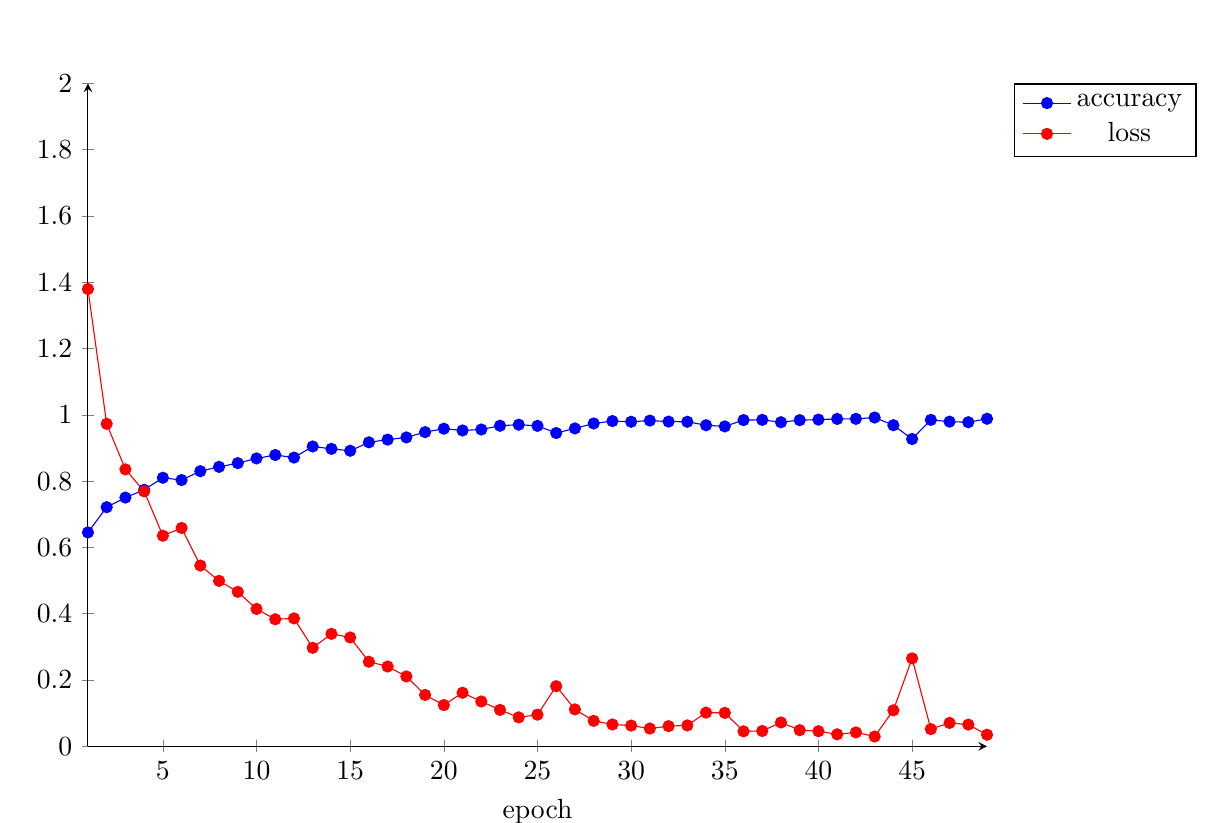
\begin{tikzpicture}
    \begin{axis}[
        width=13cm, height=10cm,
        ymin=0, ymax=2,
        xmin=1, xmax=49,
        axis x line=bottom,
        axis y line=left,
        xlabel=epoch,
        title={},
        axis on top=true, clip=false,
        legend pos=outer north east
    ]
    \addplot[mark=*, blue] coordinates {
        (1, 0.6453) (2, 0.7215) (3, 0.7505) (4, 0.7739) (5, 0.8103) (6, 0.8033) (7, 0.8301) (8, 0.8431) (9, 0.8544) (10, 0.8686) (11, 0.8789) (12, 0.8712) (13, 0.9047) (14, 0.8975) (15, 0.8917) (16, 0.9172) (17, 0.9254) (18, 0.9320) (19, 0.9479) (20, 0.9583) (21, 0.9530) (22, 0.9559) (23, 0.9672) (24, 0.9704) (25, 0.9669) (26, 0.9453) (27, 0.9591) (28, 0.9741) (29, 0.9813) (30, 0.9792) (31, 0.9828) (32, 0.9797) (33, 0.9792) (34, 0.9688) (35, 0.9652) (36, 0.9843) (37, 0.9850) (38, 0.9779) (39, 0.9841) (40, 0.9857) (41, 0.9878) (42, 0.9880) (43, 0.9920) (44, 0.9689) (45, 0.9272) (46, 0.9849) (47, 0.9796) (48, 0.9779) (49, 0.9883)
    };
    \addplot[mark=*, red] coordinates {
        (1, 1.3797) (2, 0.9730) (3, 0.8356) (4, 0.7694) (5, 0.6354) (6, 0.6588) (7, 0.5454) (8, 0.4992) (9, 0.4660) (10, 0.4144) (11, 0.3833) (12, 0.3860) (13, 0.2972) (14, 0.3393) (15, 0.3284) (16, 0.2552) (17, 0.2408) (18, 0.2108) (19, 0.1551) (20, 0.1244) (21, 0.1616) (22, 0.1353) (23, 0.1100) (24, 0.0873) (25, 0.0955) (26, 0.1813) (27, 0.1114) (28, 0.0768) (29, 0.0660) (30, 0.0626) (31, 0.0537) (32, 0.0609) (33, 0.0631) (34, 0.1017) (35, 0.1009) (36, 0.0452) (37, 0.0463) (38, 0.0720) (39, 0.0487) (40, 0.0456) (41, 0.0362) (42, 0.0420) (43, 0.0297) (44, 0.1087) (45, 0.2653) (46, 0.0519) (47, 0.0706) (48, 0.0655) (49, 0.0349)
    };
    \addlegendentry{accuracy}
    \addlegendentry{loss}
    \end{axis}
\end{tikzpicture}
\bigskip

Training time: 30.083333 minutes.

Final epoch performance:
\begin{itemize}
    \item Loss: 0.0349;
    \item Accuracy: 0.9883;
\end{itemize}

Test set performance:
\begin{itemize}
    \item Loss: 0.896843;
    \item Accuracy: 0.855769;
\end{itemize}

With much fewer parameters and much less training time than AlexNet we reached a result that is better than the expectations, comparable with AlexNet and with an accuracy even better.

\section*{Conclusions}

We report in a compact way the results:

\bigskip
\begin{tabular}{ | l | l | l | l | l | }
    \hline
    \textbf{Model} & \textbf{Input Shape} & \textbf{Accuracy} & \textbf{Loss} & \textbf{Training Time} \\ \hline
    \textbf{LeNet}        & 320x320 & 0.192909 & 2.202084 & 17.7m \\ \hline
    \textbf{AlexNet}      & 320x320 & 0.810096 & 1.190347 & 31.4m \\
                          & 420x420 & 0.839543 & 0.866917 & 72.5m \\ \hline
    \textbf{AndreaNet v1} & 320x320 & 0.767428 & 1.466683 & 15.7m \\
                          & 420x420 & 0.802284 & 0.999524 & 66.3m \\ \hline
    \textbf{AndreaNet v2} & 320x320 & 0.822716 & 0.988192 & 7.9m \\
                          & 420x420 & 0.829327 & 0.868631 & 33.6m\\ \hline
    \textbf{AndreaNet v3} & 320x320 & 0.844351 & 1.029947 & 14.5m \\
                          & 420x420 & 0.855769 & 0.896843 & 30.0m\\ \hline
\end{tabular}
\bigskip

As you can easily see AndreaNet v3 is the better choice for performance and for training time the choice is between it and the version 2.
This net has only 8 million parameters (with input 420x420). Lenet has 55 million parameters and AlexNet 78 million.
This allows us to train the network using less time and memory. In fact, memory is one of the biggest issues in training neural networks on a laptop.

This is a great goal for us, we created a speedy network with high performances starting from LeNet and, in the end, better even than AlexNet.

%\newpage
%\bibliography{main} 
%\bibliographystyle{ieeetr}

\end{document}
